\begin{tikzpicture}[]

\node[draw, thick, minimum height=2.5cm, minimum width=2cm, align=center, fill = Green!20] (corr_batch) {Correct};

\node[below= of corr_batch, draw, thick, minimum height=2.5cm, minimum width=2cm, align=center, fill = red!20, yshift=30pt] (incorr_batch) {Incorrect};

\node[draw, ultra thick, minimum height=5cm, minimum width=2cm, align=center, fill = none, yshift=-35pt] () {};

\node[align=center, yshift=-25pt, above= of corr_batch] () {Batch};

%\node[below= of corr_batch, draw, thick, minimum height=0.1cm, minimum width=2cm, align=center, fill = green!50, yshift=45pt] () {};
%
%\node[below= of incorr_batch, draw, thick, minimum height=0.1cm, minimum width=2cm, align=center, fill = red!50, yshift=45pt] () {};


\node[right=of corr_batch, align=center] (hist_corr) {
        \begin{tikzpicture}
            \begin{axis}[
                width=8cm, % Width of the plot
                height=3cm, % Height of the plot
                axis lines=left, % Draw x and y axes
%                xlabel={Class},
               	ylabel={Probability},
				axis line style={thick}, % Make the axes thick
                xmin=1, xmax=6.25, % x-axis range
                ymin=-0.2, ymax=1.25, % y-axis range
                domain=0:10, % Range for the function
                xtick=\empty, % Disable ticks
                xticklabels={Class 1, Class 2, Class 3, Class 4, Class 5},
                legend style={
                    at={(1.075, 0.05)}, % Position: bottom-right inside the plot
                    anchor=south east, % Align the legend to the bottom-right
                    draw=none, % Remove border around the legend
                    fill=none, % Transparent background
                    font=\small % Smaller font size
                },
                legend image post style={xscale=0.5},
                ybar interval=0.66,
            ]
            	\draw[darkgray, dash pattern=on 2pt off 1pt] (axis cs:0, 1) -- (axis cs:6, 1);
            	\draw[lightgray, dash pattern=on 0.5pt off 0.5pt] (axis cs:0, 0) -- (axis cs:6, 0);
            \addplot[fill=Green!50] coordinates {(1,0.07) (2,0.83) (3,0.02) (4,0.05) (5,0.03) (6,1)};
            \addplot[fill=black] coordinates {(1,0) (2,1) (3,0) (4,0) (5,0) (6,0)};
            
            	\draw[->, thick, Green] (axis cs:5.25, 0.03) to [out=90, in=90, looseness=1.5] (axis cs:5.75, 0);
            	\draw[->, thick, Green] (axis cs:4.25, 0.05) to [out=90, in=90, looseness=1.5] (axis cs:4.75, 0);
            	\draw[->, thick, Green] (axis cs:3.25, 0.02) to [out=90, in=90, looseness=1.5] (axis cs:3.75, 0);
            	\draw[->, thick, Green] (axis cs:2.25, 0.83) to [out=90, in=90, looseness=1.5] (axis cs:2.75, 1);
            	\draw[->, thick, Green] (axis cs:1.25, 0.07) to [out=90, in=90, looseness=1.5] (axis cs:1.75, 0);
            
            \end{axis}
        \end{tikzpicture}
    };
    
\node[above= of hist_corr, yshift=-30pt, xshift=15pt] () {Minimize $\text{CE}(\textcolor{Green}{p_i}, y_i)$};

\node[right=of incorr_batch, align=center] (hist_incorr) {
        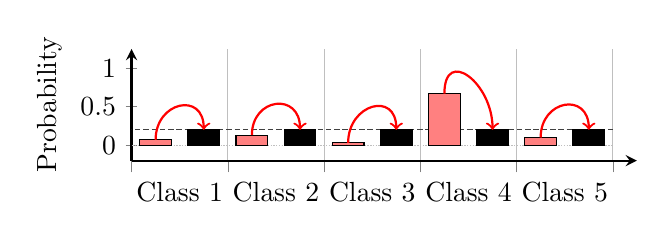
\begin{tikzpicture}
            \begin{axis}[
                width=8cm, % Width of the plot
                height=3cm, % Height of the plot
                axis lines=left, % Draw x and y axes
%                xlabel={Class},
               	ylabel={Probability},
				axis line style={thick}, % Make the axes thick
                xmin=1, xmax=6.25, % x-axis range
                ymin=-0.2, ymax=1.25, % y-axis range
                domain=0:10, % Range for the function
                xtick=\empty, % Disable ticks
                xticklabels={Class 1, Class 2, Class 3, Class 4, Class 5},
                legend style={
                    at={(1.075, 0.05)}, % Position: bottom-right inside the plot
                    anchor=south east, % Align the legend to the bottom-right
                    draw=none, % Remove border around the legend
                    fill=none, % Transparent background
                    font=\small % Smaller font size
                },
                legend image post style={xscale=0.5},
                ybar interval=0.66,
            ]
            % 	\draw[lightgray, dash pattern=on 0.5pt off 0.5pt] (axis cs:0, 1) -- (axis cs:6, 1);
            	\draw[lightgray, dash pattern=on 0.5pt off 0.5pt] (axis cs:0, 0) -- (axis cs:6, 0);
			\draw[darkgray, dash pattern=on 2pt off 1pt] (axis cs:0, 0.2) -- (axis cs:6, 0.2);
            \addplot[fill=red!50] coordinates {(1,0.07) (2,0.13) (3,0.03) (4,0.67) (5,0.1) (6,1)};
            \addplot[fill=black] coordinates {(1,0.2) (2,0.2) (3,0.2) (4,0.2) (5,0.2) (6,1)};
            
            	\draw[->, thick, red] (axis cs:5.25, 0.1) to [out=90, in=90, looseness=2.0] (axis cs:5.75, 0.2);
            	\draw[->, thick, red] (axis cs:4.25, 0.67) to [out=90, in=90, looseness=2.0] (axis cs:4.75, 0.2);
            	\draw[->, thick, red] (axis cs:3.25, 0.03) to [out=90, in=90, looseness=2.0] (axis cs:3.75, 0.2);
            	\draw[->, thick, red] (axis cs:2.25, 0.13) to [out=90, in=90, looseness=2.0] (axis cs:2.75, 0.2);
            	\draw[->, thick, red] (axis cs:1.25, 0.07) to [out=90, in=90, looseness=2.0] (axis cs:1.75, 0.2);
            	
            	
            \end{axis}
        \end{tikzpicture}
    };
    
\node[below= of hist_incorr, yshift=30pt, xshift=15pt] () {Minimize $\text{KL}\left(\textcolor{red}{p_i} \parallel \mathcal{U}\right)$};

\draw[->, thick] (corr_batch) -- (hist_corr);
\draw[->, thick] (incorr_batch) -- (hist_incorr);
	
\end{tikzpicture}